\chapter{Simulation}

\section{Method}

The stationarity of the avalanche statistic sequences forms the theoretical foundation for empirical simulation and analysis according to the following algorithm:
\needspace{5\baselineskip}
\underline{\textbf{Algorithm: Simulating the Sandpile Model}}\\
initialise $\mathbf{s}, \mathbf{a}, \mathbf{\ell}, \mathbf{d}$ as empty arrays of size $n$ \\
initialise $\eta = \mathbf{0}$\\
\textbf{for} $i \in \{1, \cdots, m \}$ \textbf{do}: \\
simulate $\mathbf{X}_i$\\
$\eta \gets \delta(\eta, \mathbf{X}_i)$\\
$\eta \gets \xi(\eta)$\\
\textbf{end for}\\
\textbf{for} $i \in \{m + 1, \cdots, m + n \}$ \textbf{do}: \\
simulate $\mathbf{X}_i$\\
$\eta \gets \delta(\eta, \mathbf{X}_i)$\\
$\mathbf{s}[i-m] \gets s(\eta)$\\
$\mathbf{a}[i-m] \gets a(\eta)$\\
$\mathbf{\ell}[i-m] \gets \ell(\eta)$\\
$\mathbf{d}[i-m] \gets d(\eta)$\\
$\eta \gets \xi(\eta)$\\
\textbf{end for}\\
\textbf{return} $\mathbf{s}, \mathbf{a}, \mathbf{\ell}, \mathbf{d}$\\

We can then discard the zero values of the returned arrays, which are not associated with an avalanche.

In the above, simulated states $\eta_1, \cdots, \eta_m$ are called burn-in states, and are discarded. After this period, we assume that the distribution of $\eta_j$ is approximately stationary. Therefore, simulations $\eta_{m+1}, \cdots, \eta_{m+n}$ are retained and their empirical distribution approximates the stationary distribution $\pi(\eta)$. From that sequence, we construct simulated sequences for each avalanche statistic of length $n$, whose distribution approximates its respective stationary distribution.

\section{Practicalities}
In practice, hundreds of thousands of simulations are required to approach stationarity. This is computationally expensive, especially for large lattice sizes, because computations cannot be parallelised due to the Markov structure of the problem. 
An initial Python implementation of the simulation procedure above was too slow to produce meaningful results. The final implementation uses \texttt{numba} with \texttt{njit} decorators, which stands for 'no python just in time' \cite{lam2015numba}. This compiles the Python code prior to execution, bypassing the CPython interpreter and achieving execution speed near code written in C. However, only a subset of Python and \texttt{numpy} functionality is permitted, requiring significant refactoring away from object-oriented design. Table \ref{tab:runtime_comparison} compares identical implementations of the simulation for varying lattice sizes, where one uses \texttt{numba @njit} decorators, while the other does not. Results show a 100-140x speedup using the optimised code.


\begin{table}
\centering
        \begin{tabular}{|l|l|l|l|}
        \hline
        $L$ & \texttt{numba}-optimised runtime (s) & standard runtime (s) & speedup\\
        \hline
            5 &  0.03 &  3.90 &  135.15 \\
            7 &  0.05 &  5.93 &  117.16 \\
            10 &  0.09 &  9.41 &  104.69 \\
            12 &  0.12 &  11.68 &  99.98 \\
            15 &  0.13 &  17.62 &  132.55 \\
        \hline
        \end{tabular}
        \caption{Runtime comparison between the \texttt{numba}-based implementation and the standard Python implementation. The optimised code runs 100-140x faster. Simulations comprised 100,000 depositions (40,000 burn-in and 60,000 subsequent) and were performed on lattice sizes $L \in \{5, 7, 10, 12, 15\}$.}
        \label{tab:runtime_comparison}
    \end{table}

\section{Results}
Simulations were performed for lattice sizes $L \in \{5, 10, 15, 20, 30, 40, 50, 65, 80, 100\}$. The burn-in period was set to $m=4\times 10^4$ and sequences of length $n=1 \times 10^6$ were retained for each lattice size.

\begin{figure}
\begin{center}
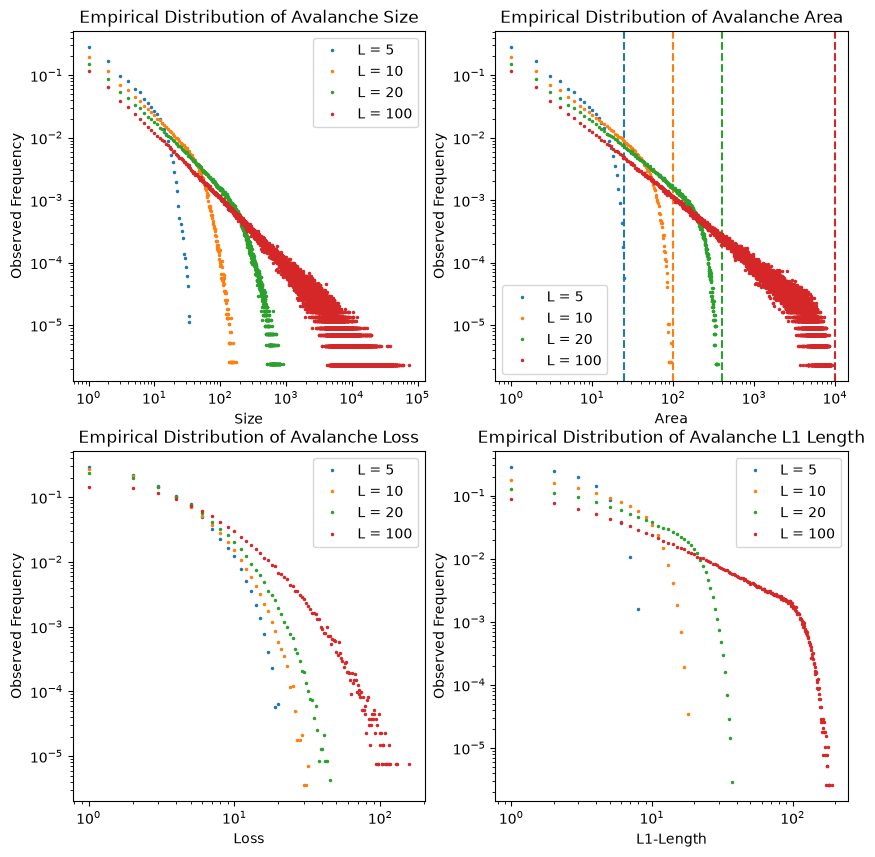
\includegraphics[width=0.80\linewidth]{figures/simulation_four_statistics.png}
\end{center}
\caption{Observed frequencies of key avalanche statistics computed from the simulated sandpile Markov chain, excluding the discarded burn-in samples. A subset of four lattice sizes are depicted: 5, 10, 20, and 100, with varying colors. Values are computed from $10^6$ simulated observations. The dashed vertical lines on the top right correspond to the maximum possible avalanche area for each lattice size, $L^2$. Plots are shown in log-log axes. The appearance of horizontal lines is an artifact of the log-log axes. The lines correspond to sizes with only 1, 2, 3, etc. observations in the dataset, with exaggerated vertical distance between the lines because of the log scale.}
\label{fig:simulation_statistics}
\end{figure} 

The plots in Figure \ref{fig:simulation_statistics} depect a linear trend in early values of avalanche size, area, and $L_1$ distance, suggesting a power law distribution followed by a sharp decay. The distribution for Loss does not appear to have this power law structure, and the remainder of this report focusses on understanding and analysing the distribution of avalanche size, area, and length.